\documentclass[11pt]{report}

\usepackage[utf8]{inputenc}
\usepackage[french]{babel}
\usepackage{fullpage}
\usepackage{graphicx}
\usepackage{fancyhdr}	% headers/footers
\usepackage{xcolor}		% to use our own color
\usepackage{lastpage}	% to easily know the total number of pages
\usepackage{titling}	% to easily know the total number of pages
\usepackage{colortbl}	% to put color in a table background
\usepackage{datetime}	% to allow us set a new date formatting
\usepackage{multirow}   % to allow multirows in tables
\usepackage[colorlinks,linkcolor=black]{hyperref}
\usepackage{palatino}
%% \usepackage[colorlinks=false, urlcolor=blue, breaklinks, pagebackref, citebordercolor={0 0 0}, filebordercolor={0 0 0}, linkbordercolor={0 0 0}, pagebordercolor={0 0 0},
%%                      runbordercolor={0 0 0}, urlbordercolor={0 0 0}, pdfborder={0 0 0}]{hyperref}

% Custom defines zone

% Define useful hand-made colors
\definecolor{epiBlue}{RGB}{0,110,255}
\definecolor{lightGray}{gray}{0.92}

% Bit of code to bold an entire table row
% http://tex.stackexchange.com/questions/4811/make-first-row-of-table-all-bold
\newcolumntype{$}{>{\global\let\currentrowstyle\relax}}
\newcolumntype{^}{>{\currentrowstyle}}
\newcommand{\rowstyle}[1]{\gdef\currentrowstyle{#1}%
  #1\ignorespaces
}

% Defining a "dd/mm/yyyy" date format
\newdateformat{dashDate}{\twodigit{\THEDAY}/\twodigit{\THEMONTH}/\twodigit{\THEYEAR}}

% Define Document Title
\newcommand{\ProjectTitle}{Onitu}
\newcommand{\DocTitle}{EIP Onitu}
\newcommand{\SubTitle}{Bilan Architecure AA1}

% Defining some logo image names
\newcommand{\ProjectLogo}{}
\newcommand{\EIPLogo}{logo_eip.png}

% Setting the space between each page's header and its content
\setlength{\headsep}{0.2in}

% end of Defines


% fancyhdr-specific commands
\setlength{\headheight}{15.2pt}

%% Defining headers and footers contents.

% Big dirty hack of the "empty" pagestyle to show header and footer on the title page (in wait of a better solution)
\fancypagestyle{empty}
{
	\renewcommand{\headrulewidth}{0pt}
	\renewcommand{\footrulewidth}{1pt}
	\fancyhead[L]{\includegraphics[height=35pt]{\EIPLogo}}
	\fancyhead[C]{}
	\fancyhead[R]{\textcolor{epiBlue}{\textbf{\emph{\huge{\ProjectTitle}}}}}

	\fancyfoot[L]{}
	\fancyfoot[C]{\textcolor{epiBlue}{\textbf{\underline{\DocTitle\ — \SubTitle}}}}
	\fancyfoot[R]{}
}

\fancypagestyle{EIP}
{
	\renewcommand{\headrulewidth}{0pt}
	\renewcommand{\footrulewidth}{1pt}
	\fancyhead[L]{\includegraphics[height=35pt]{\EIPLogo}}
	\fancyhead[C]{}
	\fancyhead[R]{\textcolor{epiBlue}{\textbf{\emph{\huge{Onitu}}}}}

	\fancyfoot[L]{\textcolor{epiBlue}{\textbf{\underline{\leftmark}}}}
	\fancyfoot[C]{}
	\fancyfoot[R]{
		\thepage/\pageref{LastPage}
	}
}

\pagestyle{EIP} % does not seem to work ...

% end of fancyhdr stuff

%Gummi|063|=)

%\title{The Title\\\normalsize A Sub-title}
\title{
	\huge{\textbf{\textcolor{epiBlue}{\DocTitle} } }\\
	\Large{\textbf{\emph{\textcolor{gray}{\SubTitle} } } }
}


\begin{document}
\addtocontents{toc}{\protect\refstepcounter{page}} % makes the table of contents count pages from 1 (one)
\maketitle

\thispagestyle{empty}
\vspace*{10mm}

\textbf{\emph{\textcolor{onitu}{\large{Résumé du document} } } }\\

Résumé !!!

\clearpage


\thispagestyle{empty}
\vspace*{10mm}
\textbf{\emph{\textcolor{epiBlue}{\large{Description du document} } } } \\

\vspace*{2mm}

\begin{tabular}{|>{\columncolor{epiBlue} \color{lightGray} \bfseries } l|l|}
\hline
	Titre & \DocTitle\\
\hline
	Date & \dashDate\today \\
\hline
	Auteur & Alexandre BARON\\
\hline
	Responsable & Louis Roché\\
\hline
	E-Mail & onitu\_2015@labeip.epitech.eu\\
\hline
	Sujet & Ceci n'est pas un template\\
\hline
	Mots clés & Mot, clé\\
\hline
	Version du modèle & 2.1\\
\hline
\end{tabular}

\vspace*{10mm}

\textbf{\emph{\textcolor{epiBlue}{\large{Tableau des révisions} } } }\\

\vspace*{2mm}

\begin{tabular}{|$l|p{4cm}|p{2cm}|p{5cm}|}
\hline
\rowcolor{epiBlue}
\rowstyle{ \color{lightGray} \bfseries}
	Date & \textcolor{lightGray}{\textbf{Auteur}} & \textcolor{lightGray}{\textbf{Section(s)}} & \textcolor{lightGray}{\textbf{Commentaires}}\\
\hline
	18/05/2013 & Antoine Rozo & Chapitre 1 & Ajout de l'introduction \\
\hline
	20/05/2013 & Antoine Rozo & Chaptire 2 & Architecture, buts et contraintes \\
\hline
\end{tabular}

\tableofcontents
\addtocontents{toc}{\protect\thispagestyle{empty}
                    \protect\pagestyle{empty}}
\thispagestyle{empty}

\chapter{Rappel de l'EIP}
\thispagestyle{EIP} % seems mandatory
\setcounter{page}{1} %reset the page count

\section{Qu'est-ce qu'un EIP et Epitech}
Epitech, école d'expertise informatique en cinq ans, offre aux étudiants l'opportunité de réaliser un projet de fin d'études sur trois ans, l'EIP (pour \emph{Epitech Innovative Project}).\\

À ce titre, les élèves doivent s'organiser en un groupe d'au moins cinq personnes et choisir un sujet porteur de nouveautés ou améliorant un ancien sujet. L'EIP est un passage obligatoire et unique dans la scolarité de l'étudiant, de par son envergure (18 mois) et la préparation requise. Le but est, à la fin du temps imparti, d'obtenir un projet commercialisable.


\section{Principe de base du système futur}
    Onitu est un projet visant à proposer une implémentation libre et Open Source du serveur d’Ubuntu One.\\

    Ubuntu One est un service de Canonical (sponsor officiel d'Ubuntu) permettant de disposer d’un espace de stockage en ligne qui sera synchronisé entre différents ordinateurs et périphériques compatibles via un logiciel client. Le client et le protocole d’Ubuntu One sont disponibles sous licence libre. Néanmoins, le serveur est propriétaire et n’a pas été publié.\\

    L'objectif d'Onitu de proposer un équivalent libre à ce serveur, afin de profiter des fonctionnalités d’Ubuntu One tout en maîtrisant le stockage des données et des informations.\\

    Les fichiers gérés par Onitu pourront être stockés sur un serveur administré par un utilisateur, ou bien sur des services tiers comme Dropbox, Amazon S3, ou Google Drive.\\

    La cible première d'Onitu est l'utilisateur averti, soucieux des problématiques de centralisation des données, et son entourage, à qui il fera profiter le serveur mis en place. Il n'est pas forcément technicien mais assez curieux, le profil même de l'utilisateur Ubuntu.
    Onitu vise aussi à être utilisé au sein d'entreprises ayant la volonté de maîtriser facilement le stockage de leur données.\\

\section{Abréviations, anglicismes, acronymes}

\begin{itemize}
\itemsep1pt\parskip0pt\parsep0pt
\item
  \emph{driver}: Module se greffant au programme et permettant la
  gestion d'un service de stockage.
\item
  \emph{core}: Cœur du programme, module principal.
\item
  \emph{DSL (Domain Specific Language)}: Langage de programmation dédié
  à un domaine précis.
\end{itemize}

\section{Références}


\chapter{Architecture, buts et contraintes}
\thispagestyle{EIP} % seems mandatory

\section{Objectifs spécifiques ayant un impact sur l'architecture}

La réflexion sur l'architecture du projet passe d'abord par la
définition d'objectifs clairs, que voici énoncés.

Le premier objectif est d'offrir une alternative libre au serveur
\emph{Ubuntu One}, et donc d'être entièrement compatible avec ce
dernier.

Un autre est d'offrir à l'utilisateur un contrôle total sur ses données,
il lui revient de choisir où ses fichiers seront stockés.

Aussi, pour une meilleure expérience utilisateur, cette solution se
devra d'être facilement déployable.

Un des objectifs est aussi de permettre de stocker les données sur des
services externes, tels \emph{Dropbox}, par l'intermédiaire de
\emph{drivers}. C'est principalement autour de cet objectif que se forme
l'architecture du projet.

\section{Contraintes fonctionnelles}

Différentes contraintes permettent aussi de diriger les choix
techniques. Premièrement, les contraintes fonctionnelles, qui décrivent
les caractéristiques du système.

Il a été décidé que les différents \emph{drivers} communiqueraient
entre-eux à l'aide de queues de messages. Ainsi, le programme disposera
d'un \emph{core} très basique, ne s'occupant que de la transmission des
messages.

Une autre contrainte et la volonté de pouvoir assurer une réplication
des données sur différents services. Par l'intermédiaire des
\emph{drivers}, préalablement configurés, qui écouteront les
modifications d'un ensemble de fichiers pour les reproduire à
l'identique sur leur espace de stockage.

L'ensemble des modules devront pouvoir être configurés de façon
centralisée à l'aide d'un \emph{DSL}, permettant une configuration plus
souple qu'un simple système clef-valeur.

\section{Contraintes non fonctionnelles}

Les autres contraintes, non fonctionnelles, régissant les choix
architecturaux sont les suivantes.

Onitu devra être conforme au protocole définit par \emph{Ubuntu One},
puisque compatible avec le client officiel.

L'utilisation de certaines bibliothèques, telles que \emph{Twisted}, non
portée en Python3, contraint à l'utilisation d'une version antérieure.

Dans un soucis de simplicité, le \emph{DSL} proposé devra être
facilement compréhensible par l'utilisateur, ne devra pas le rebuter. Ce
dernier devrait sans problème pouvoir bénéficier d'une configuration
fine de son système.

C'est principalement dans un soucis de protection et contrôle des
données que la solution Onitu sera utilisée, c'est pourquoi sa sécurité
doit être maximale.


\chapter{Représentation de l’architecture globale}
\thispagestyle{EIP}

\section{Schématisation}
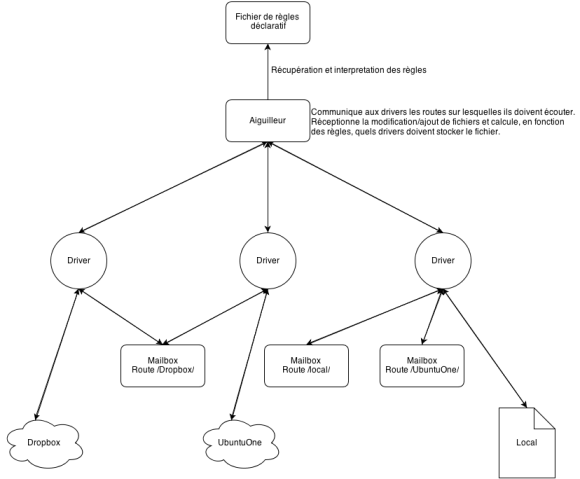
\includegraphics{schema_architecture_globale.png} 

\newpage
\section{Fichier de règles}

Le fichier de règles permet à l'utilisateur de configurer les choses suivantes:
\newline

\begin{itemize}
\itemsep1pt\parskip0pt\parsep0pt
\item
  Le nombre de répliques d'un fichier/dossier (À combien d'endroits il doit être stocké).
\item
  L'endroit où un fichier doit obligatoirement être stocké.
\item
  L'endroit où un fichier ne doit pas être stocké.
\newline
\end{itemize}

La définition de ces règles par l'utilisateur est facultative, Onitu a une configuration de base, completée et/ou modifiée par ce fichier.


\section{L'aiguilleur}
L'aiguilleur interpréte ce fichier, c'est lui qui donne l'ordre à un \emph{driver} d'écouter ou de ne plus écouter sur une route.
Il va également recevoir des messages de \emph{drivers} lui indiquant la création/suppression/mise à jour de certains fichiers, son rôle dans ce cas est d'informer les \emph{drivers} concernés de ce qu'ils doivent faire (écouter sur une nouvelle route par exemple).


\section{Les drivers}
Le rôle d'un \emph{driver} est d'assurer le CRUD (Create, Read, Update, Delete) des fichiers sur la plateforme de stockage qui lui est destinée (Local/UbuntuOne/Dropox etc).
C'est les \emph{drivers} qui réalisent la liaison entre Onitu et les différents services de stockage.


\section{Gestion de la communication entre les modules}
La communication entre les différents composants (\emph{drivers/aiguilleur}) se fera à l'aide d'un système de message fiable et rapide appelé ZeroMQ. Ce sont les \emph{mailbox} représentées sur le shéma qui contiendront ces messages.



\chapter{Taille et performance}
\thispagestyle{EIP} % seems mandatory

\section{Environnement}

Onitu est destiné à être utilisé avant tout dans un cadre privé par des particuliers. Par conséquent, nous avons des dispositions particulières à prendre car les contraintes ne sont pas les mêmes.

Tout d'abord, les machines sur lesquelles Onitu va être installé seront très diverses et risquent de varier entre entrée de gamme et serveur professionnel. Nous devrons donc prévoir une installation facilitée, et qui s'adapte aux capacités du serveur. Le lancement des différents services et leur administration devront également être simples, de façon à pouvoir être utilisés par n'importe quel utilisateur (amateur ou professionnel).

Bien que nous nous concentrions principalement sur Linux, il nous semble important d'être portable. Nous ferons donc le nécessaire pour que le portage demeure facile lorsque le projet sera plus avancé.

\section{Stockage}

Concernant les performances d'Onitu, elles seront principalement évaluées sur deux points principaux: le stockage et les réponses aux requêtes utilisateur.

En ce qui concerne le stockage, nous devrons faire face à un nombre potentiellement très grand de fichiers. Nous avons donc choisi une architecture simple, qui puisse fonctionner en plusieurs instances. De cette façon, le système est extensible et pourra ainsi fournir un espace de stockage virtuellement illimité, à condition d'avoir les ressources nécessaires.

L'organisation et l'équilibrage interne peuvent se faire sur des périodes de temps plus longues et régulières.

\section{Accès}

Dans un usage typique du produit, nous aurons relativement peu d'utilisateurs et de requêtes simultanés. En effet, une instance Onitu étant principalement destinée à un usage privé ou en entreprise, elle aura un nombre réduit d'utilisateurs, au maximum le nombre d'employés d'une petite entreprise, c'est-à-dire quelques dizaines de personnes.

Ces utilisateurs ne feront pas beaucoup d'opérations simultanées. Nous estimons que nous aurons moins de quelques centaines de requêtes par heure, avec des pics à quelques dizaines. Ces chiffres sont très raisonnables pour un serveur, et ne poseront donc pas de problèmes.

Dans un projet comme Onitu, la difficulté est que les requêtes individuelles peuvent être lourdes, car il s'agira souvent de transfert de fichiers entre un des drivers et le client. Dans la mesure du possible, ces requêtes seront redirigées directement vers le driver concerné, évitant ainsi une surcharge du serveur en façade.

Il est primordial que les requêtes ne soient pas bloquantes et s'effectuent rapidement. Pour cela, nous avons choisi d'effectuer certaines actions de manière asynchrone. Par exemple, la mise à jour des drivers et la redistribution des fichiers en fonction de la charge de chaque plateforme de stockage seront faites en parallèle, indépendamment de quand les requêtes utilisateur sont faites.



\chapter{Qualité}
\thispagestyle{EIP} % seems mandatory

Notre architecture devra répondre à plusieurs problématiques autre que les contraintes purement fonctionnelles.

Comme abordé dans la partie Taille et performance, nous avons une charge réseau atypique. Nous n'aurons pas à faire face à un grand nombre de requêtes, mais chacune sera potentiellement relativement lourde et longue. La solution choisie est de favoriser le plus possible les échanges directs entre les clients et les drivers, lorsque c'est possible.

Nous devrons aussi répondre aux exigences des utilisateurs, notamment concernant la sécurité de leur données et notre capacité à faire face à des pertes sur certains drivers ou l'indisponibilité de ceux-ci. Pour cela, nous avons un système d'aiguilleur paramétrable dont le travail sera de faire en sorte que l'état d'Onitu corresponde à celui décrit dans le fichier de configuration. De cette façon, l'utilisateur pourra définir, par un ensemble de règles, le nombre de sauvegardes des fichiers et les priorités des drivers.

Onitu devra également avoir d'autres qualités qui sont attendues d'un système semblable. Tout d'abord, nous devrons assurer la confidentialité des données et l'authentification. Pour cela, nous utiliserons des protocoles déjà en place et reconnus, tel que OAuth.

En ce qui concerne les différents drivers servant à la gestion du stockage de fichiers dans  Onitu, la sécurité de leurs protocoles respectifs ne dépend pas de nous. Nous ne pourrons que conseiller l'utilisateur sur la configuration de la solution en fonction de ses attentes, (confidentialité, intégrité, authentification…), par exemple en lui conseillant \textit{SFTP} au lieu de \textit{FTP}.

La fiabilité du système est aussi très importante, et sera assurée par une conception simple et modulaire. Si l'un des drivers a un problème, cela n'impactera pas le fonctionnement global du système et devrait être transparent pour l'utilisateur si des alternatives sont possibles, par exemple si nous avons des sauvegardes du fichier demandé sur un autre driver.

La portabilité sera assurée principalement par Python. C'est le langage principal utilisé dans Onitu et il est présent sur tout les principaux systèmes d'exploitation. Nous prêtons une attention particulière aux modules et aux bibliothèques que nous utilisons pour nous assurer un portage facile.



\end{document}
